\section{Evaluation}
\label{sec:eval}
We evaluate the accuracy of HashFilter through a series of simulations in which we fine tune the various parameters: number of stages, memory size, hash functions vs. random assignment, and probabilistic admission coefficients. In order to simulate realistic streams of traffic, we ran testing using three different traces from the equinox chicago ISP backbone link, recorded in 2016. These anonymized traces each contain between 20 - 40 million packets, over 1 million different flows, and range from 40 minutes to 1 hour long. The data was obtained with permission from the Center for Applied Internet Data Analysis (CAIDA)~\cite{caida}. We parsed the data from the CAIDA traces to isolate only the source IP addresses. Each source IP address is considered a separate flow.
\subsection{Accuracy Metrics}
Through measuring the false negative rate when testing our algorithms against the CAIDA data, we attempted to experimentally determine which combination of design policies yielded the best results. We focused on testing the two different admission policies, and applied different levels of randomized slot assignment to find an optimal algorithm. When applying front rejection, we found that uniformly randomizing the table index only in the first stage yielded the best results, and gave as much as a 50 percent accuracy improvement over simple front rejection with normal hashing (see Figure~\ref{fig:bouncer}). While some randomization provided improvements for front rejection, our tests of back rejection showed that normal hashing at all stages was best (see Figure~\ref{fig:interview}).
\begin{figure}[!htb]
  \centering
    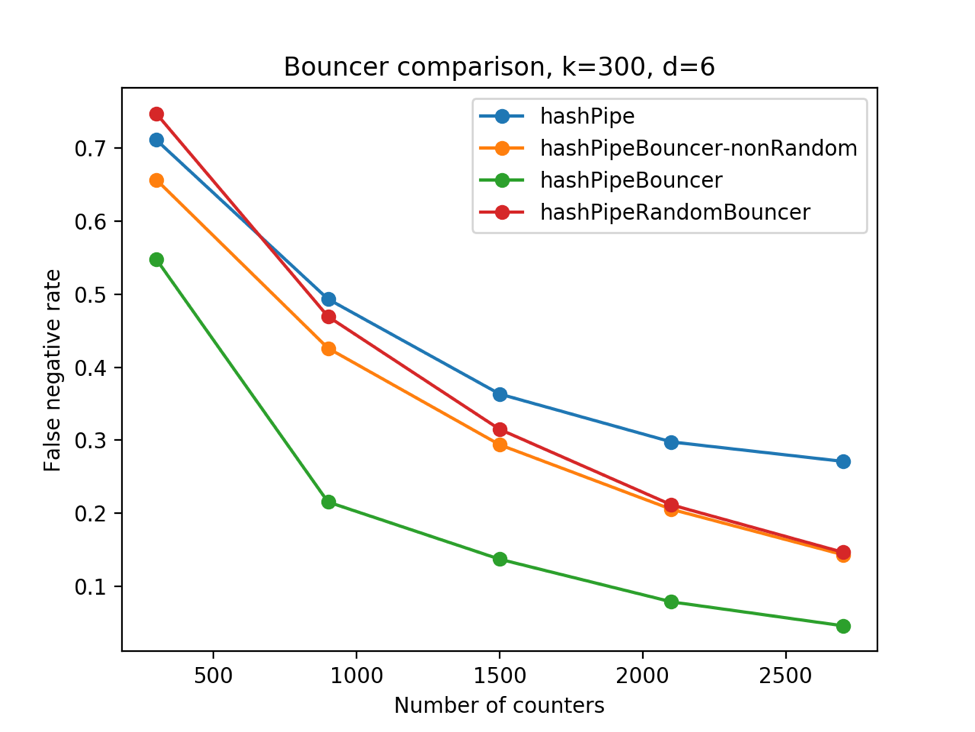
\includegraphics[scale=0.5]{bouncer}
     \caption{Comparison of Bouncer admission policy algorithm with different combinations of randomization and hashing at each stage. In hashPipeBouncer-nonRandom, consistent hash functions are used in every stage, and no randomness is applied. The hashPipeBouncer algorithm only applies randomness in the first stage. This variation performed best across all memory sizes and is the main Bouncer algorithm we use in further comparison. The hashPipeRandomBouncer algorithm uses randomness in all stages.}
     \label{fig:bouncer}
\end{figure}
\begin{figure}[!htb]
  \centering
    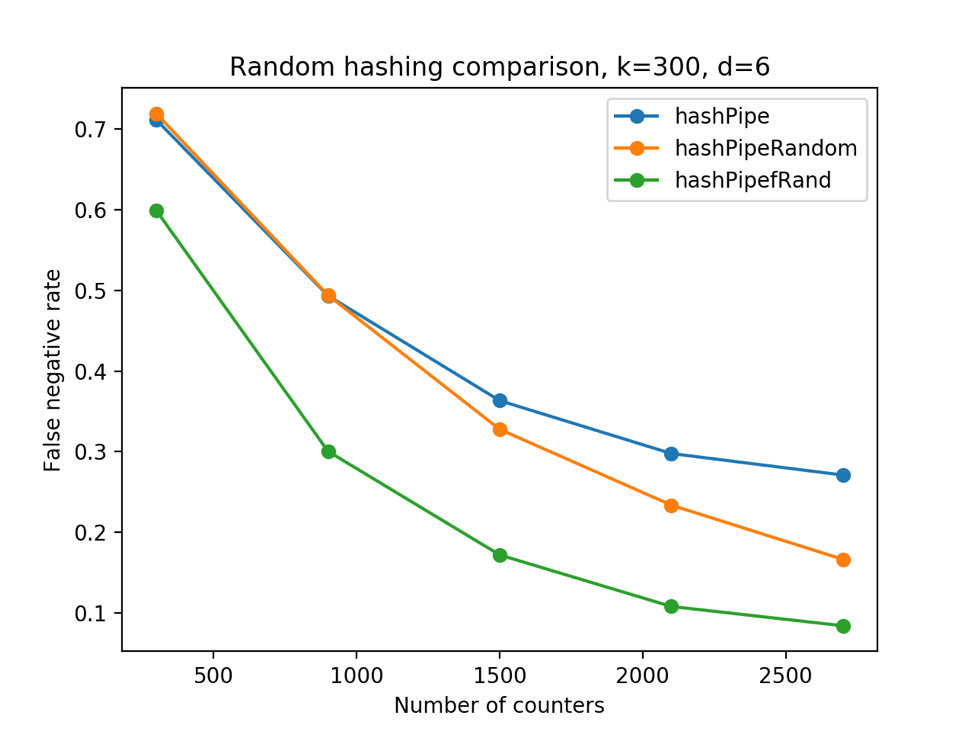
\includegraphics[scale=0.5]{interview}
     \caption{Impact of random assignment versus hash functions. The hashPipeRandom algorithm randomizes indices in all stages and provides some benefits at high memory sizes. The hashPipefRand algorithm assigns a random index in the first stage and then uses consistent hash functions in the following stages. Randomization in the first stage improves accuracy rates across the entire tested memory range, showing that randomization is useful absent any strict admission policy.}
     \label{fig:interview}
\end{figure}
Why is there a discrepancy in the effectiveness of random slot assignment? Perhaps this can be explained by the increased level of eviction that occurs in the first stage when random indices are used. When slot assignments are randomized, it is less likely that the same key will end up at the same index and increase its count in the first stage. So effectively, keys are more quickly pushed to later stages where there is a greater emphasis on retaining heavy flows. Since consistent hashing is performed in later stages, the same key is able to add to its count, and can do this more frequently when it is quickly sent down the pipeline from the first stage. Randomized slot assignment more effectively treats the first stage as transient, so light flows will more quickly be evicted and heavy flows will more quickly be retained in the core of the pipeline. For this reason, randomizing indices in all stages is less effective because retention also is lower in the latter stages, when it is most important to hold onto heavy flows. Randomization in the first stage adds an accuracy boost to front rejection, but it introduces problems with the more complex back rejection policy. The goal with the Interview policy, is to deny first stage admission to the incoming key at a high rate, and replace it with the probabilistic minimum that emerges from the pipeline. However, when randomization is applied, we can't guarantee that we are swapping the minimum with the incoming key in the first stage. This renders our stricter admission policy ineffective if we can't guarantee that the incoming key is the one being evicted in the first stage. Evidently, randomized slot assignment in the first stage can effectively increase accuracy under the right conditions, and was even shown to be useful as a standalone improvement to HashPipe without applying front or back rejection (see Figure~\ref{fig:random}). However, front rejection does not benefit from randomized slot assignment, and the standalone version of the policy ended up with the best performance. In all further testing when randomization is applied, we run multiple trials on each dataset and report average values.
\begin{figure}[!htb]
  \centering
    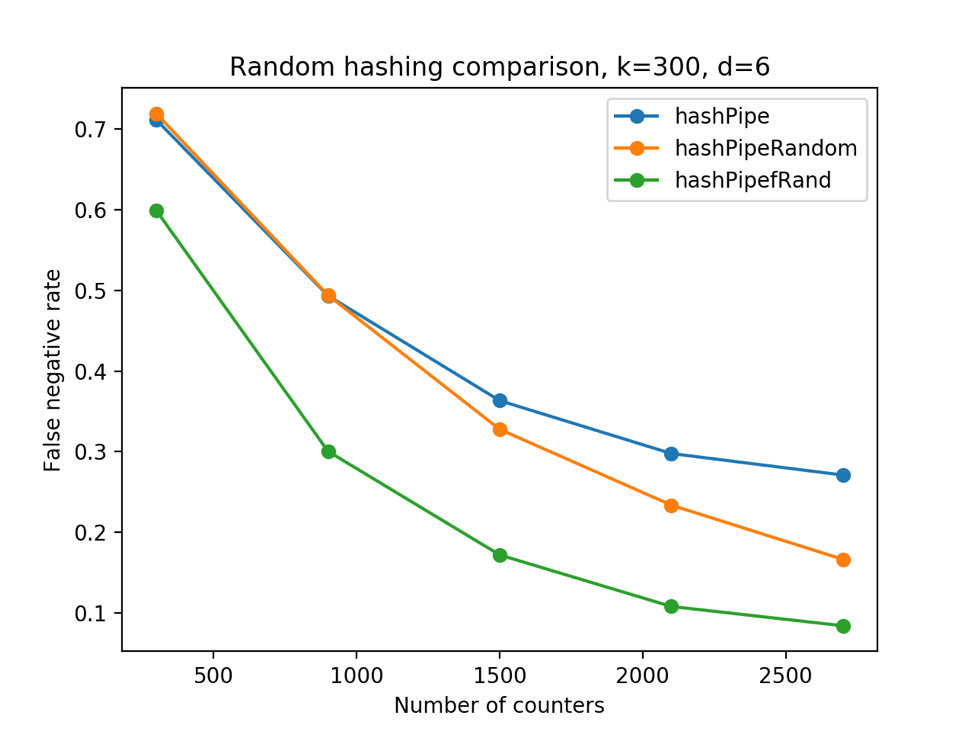
\includegraphics[scale=0.5]{random}
     \caption{Impact of random slot assignment versus hash functions. The hashPipeRandom algorithm randomizes indices in all stages and provides some benefits at high memory sizes. The hashPipefRand algorithm only hashes to a random index in the first stage and then uses consistent hash functions in the following stages. Randomization in the first stage improves accuracy rates across the entire tested memory range, showing that randomization is useful absent any strict admission policy.}
     \label{fig:random}
\end{figure}
We were also able to tune our algorithm's performance by experimenting with the multiplicative factor in our logarithmic admission equation. Figure~\ref{fig:log} shows how performance improved up to a log factor value of 5, and experienced diminishing returns thereafter. We settled on using a log factor of 5 for both front and back rejection admission policies for all further HashFilter testing.
\subsection{Comparison of HashPipe Implementations}
We began algorithm comparison by varying the available memory size, which corresponds to a greater number of counters that can be stored across all hash tables. Figure~\ref{fig:falsenegatives} shows our results when searching for the top 300 flows and using 6 table stages. Both algorithms that applied an admission policy outperformed the standard HashPipe algorithm for all tested memory sizes. Accuracy rates improved by about 20 percent when the number of counters was limited to 300, equal to the number of top-$k$ flows being identified, and increases to more than 50 percent improvement when more than 2000 counters are used. HashPipe with front rejection in particular brought its accuracy rate to more than 90 percent with 2000 counters, which is less than half the memory required by the standard HashPipe algorithm to achieve that accuracy with 300 heavy hitters and 6 table stages. In all algorithms, improvement begins to diminish after 1000 counters are available.
\begin{figure}[!htb]
  \centering
	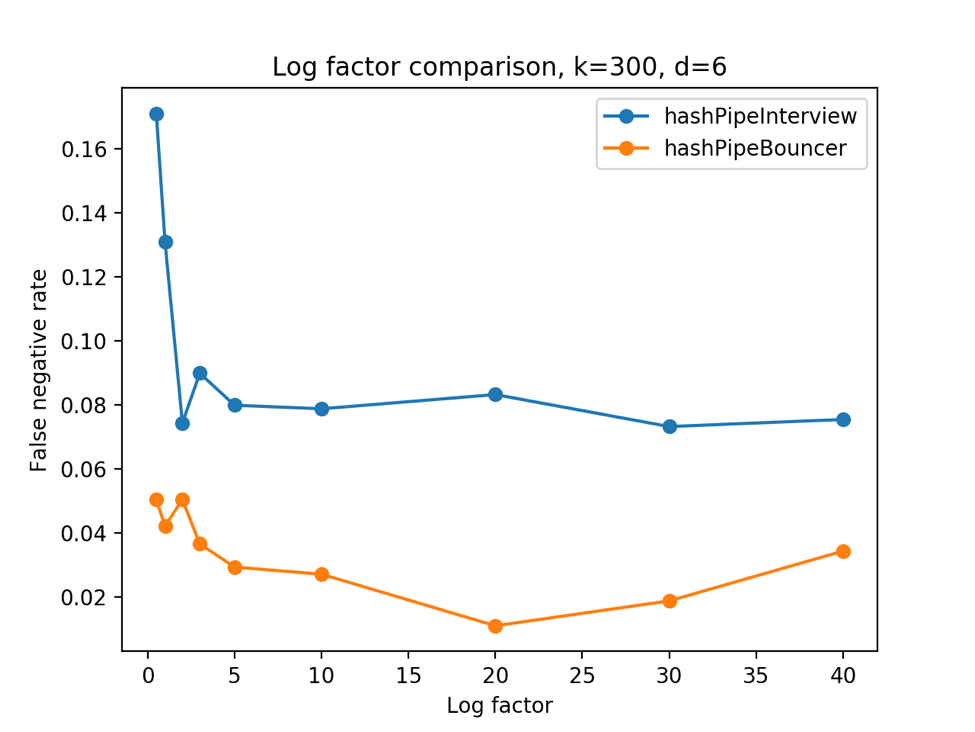
\includegraphics[scale=0.5]{log}
     \caption{Impact of varying the factor f when calculating the admission threshold $p = 1 / (f*log(c_m + 1))$. Results show that factors of 5 and greater experienced relatively similar accuracy rates for both front rejection and back rejection.}
     \label{fig:log}
    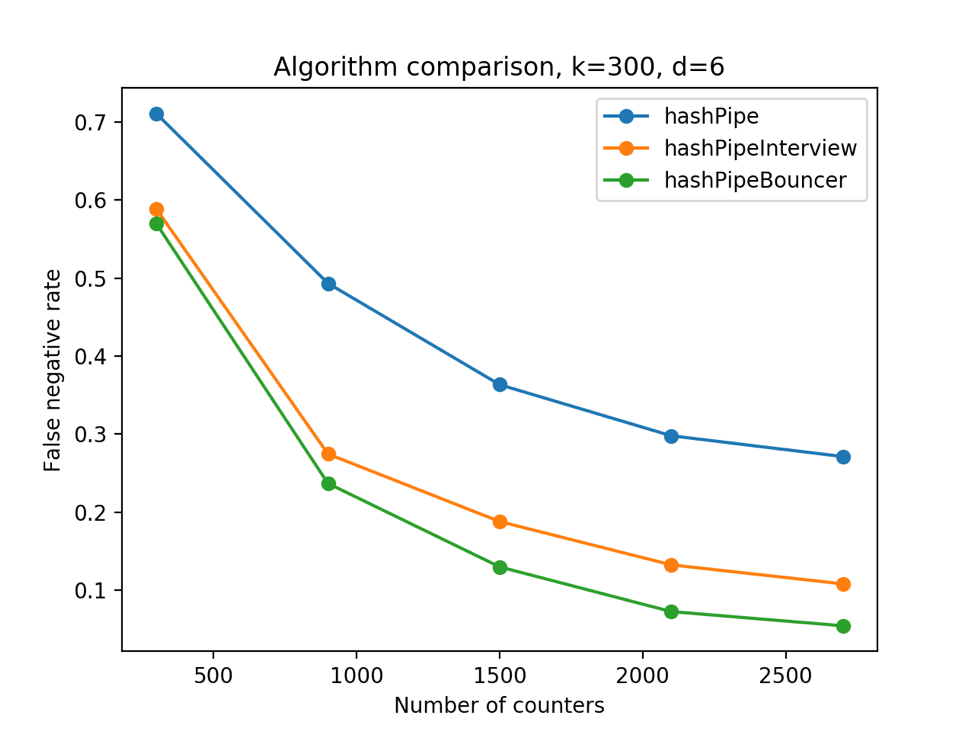
\includegraphics[scale=0.5]{falsenegatives}
     \caption{Comparison of false negatives of Interview and Bouncer to baseline. Both algorithm optimizations improve on the standard HashPipe algorithm over the entire tested memory range.}
     \label{fig:falsenegatives}
\end{figure}
In addition to testing the impact of varying memory, we also experimented with the number of pipeline stages available. HashPipe tends to perform best with a limited amount of stages so that the number of duplicates is limited. The optimal number of stages is about 6 with the standard HashPipe, but Figure~\ref{fig:stageComparison} shows that our algorithms continue to improve past this point as the number of table stages is increased. While Interview and Bouncer also experience diminishing returns after about 8 table stages, they do not see the same performance decrease present in the standard HashPipe algorithm.
\begin{figure}[!htb]
  \centering
    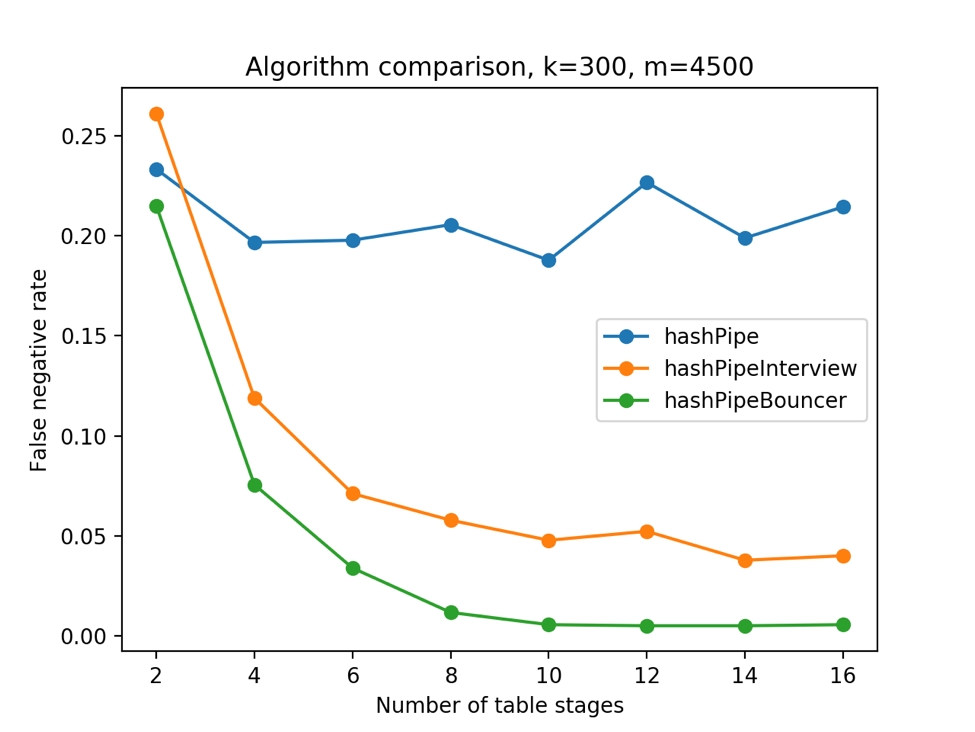
\includegraphics[scale=0.5]{stageComparison}
     \caption{Comparison of algorithms when number of table stages is varied. Interview and Bouncer do not suffer from the same accuracy drawbacks as the baseline when increasing the number of table stages.}
     \label{fig:stageComparison}
\end{figure}
\subsection{Space Saving Comparison}
As a final benchmark, we compare both variants of HashFilter to the Space Saving algorithm, which finds the true minimum of all of its counters. While this algorithm allows for more accuracy, hardware constraints preventing writes based off of multiple reads make implementations of this algorithm unrealistic. Figure~\ref{fig:spacesaver} shows that our algorithms fall behind an idealized implementation of Space Saving, where it is no issue to compute a global minimum. Similar to the baseline implementation of HashPipe, our implementations also outperform Space Saving when a low amount of memory is available. This is because Space Saving is only guaranteed to hold onto the $k$th heaviest item when it is larger than average count in the table, so its full benefits are realized when memory is increased
\begin{figure}[!htb]
  \centering
    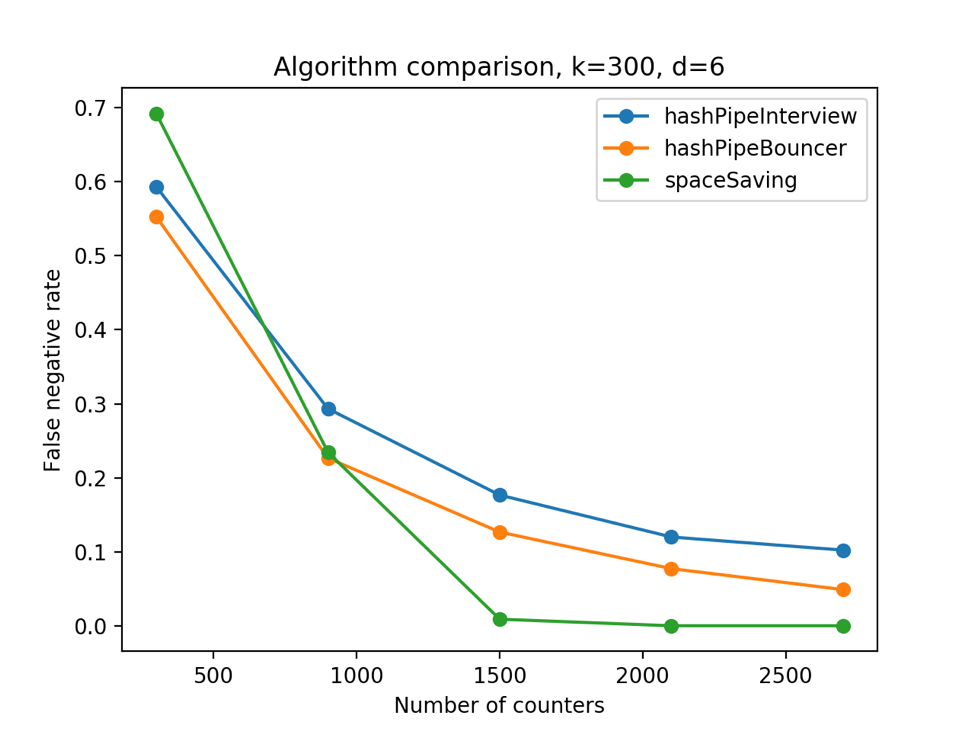
\includegraphics[scale=0.42]{spacesaver}
     \caption{Comparison of Interview and Bouncer with Space Saving with number of counters varied.}
     \label{fig:spacesaver}
\end{figure}